\documentclass[modern]{aastex61}
\usepackage{graphicx}
\usepackage{grffile}
\usepackage{xcolor}
\usepackage[sort&compress]{natbib}
\usepackage[hang,flushmargin]{footmisc}
\usepackage{amsmath}

% units macros
\newcommand{\unit}[1]{\mathrm{#1}}
\newcommand{\km}{\unit{km}}
\newcommand{\m}{\unit{m}}
\newcommand{\s}{\unit{s}}
\newcommand{\kms}{\km\,\s^{-1}}
\newcommand{\ms}{\m\,\s^{-1}}
\newcommand{\ang}{\text{\normalfont\AA}}

% math macros
\newcommand{\dd}{\mathrm{d}}
\newcommand{\T}{^{\mathsf{T}}}

% text macros
\newcommand{\todo}[1]{\textcolor{red}{#1}}  % gotta have \usepackage{xcolor} in main doc or this won't work
\newcommand{\acronym}[1]{{\small{#1}}}
\newcommand{\project}[1]{\textsl{#1}}
\newcommand{\RV}{\acronym{RV}}
\newcommand{\CRLB}{\acronym{CRLB}}

\setlength{\parindent}{1.4em} % trust in Hogg

\shorttitle{is spectro-perfectionism perfect?}
\shortauthors{smartasses}

\begin{document}\sloppy\sloppypar\raggedbottom\frenchspacing % trust in Hogg
\graphicspath{ {figures/} }
\DeclareGraphicsExtensions{.pdf,.eps,.png}

\title{How perfect is spectro-perfectionism, really?}

\begin{abstract}\noindent
Within the exoplanet community, spectrographs and their data reduction pipelines are designed with a primary goal in mind: obtaining the most precise radial velocity (\RV) measurement possible. 
In some cases, design decisions are made at the instrument level to sacrifice some degree of spectrograph throughput (?) for the sake of being able to extract a reliably calibrated spectrum from the data without losing much of the \RV\ information it encodes. 
The concept of ``spectro-perfectionism'' (cite) outlines a way to extract spectra without information loss from any reasonable spectrograph design, at least in principle. 
In this work we test the performances of traditional optimal extraction and of spectro-perfectionism on simulated spectra under a variety of spectrograph conditions. 
We find that under [x] conditions, spectro-perfectionism is able to extract precise \RV s [at/near the Cram\'er--Rao bound], outperforming optimal extraction [by a factor of...]. 
However, both methods begin to fail when [x], suggesting a future need for fully two-dimensional \RV\ extraction pipelines.
\end{abstract}

\section{Introduction}

Background on EPRV instruments and assumptions they make.

Background on optimal extraction and spectro-perfectionism

What we set out to do

\section{Data Generation}
General concept is a `photon-based' approach, meaning that a 2D spectrum is generated by repeating the following steps many times:
\begin{enumerate}
    \item select a random position in the input slit/fiber using a PDF that reflects the slit/fiber format.
    \item select a random wavelength (using the spectral source that we want to simulate as a PDF)
    \item transformation of the input position to a detector position via a (wavelength-dependent) affine transformation matrix.
The matrix represents (part of) the spectrograph optics and adjusting the matrix elements allows to define linear dispersion, the spatial format of the 2D spectrum as well as slit rotation ($\Theta$), shear and scaling (sx, sy) in dispersion and cross-dispersion direction.
    \item select a random xy distortion using a Gaussian (for now!) distribution to represent the spectrographs PSF
    \item bin the resulting detector position into detector pixels
\end{enumerate}
In equations:\\
Using

   	\[
	M_{\lambda} = \begin{pmatrix} m_{00} & m_{01} & m_{02} \\ m_{10} & m_{11} & m_{12} \\ m_{20} & m_{21} & m_{22} \end{pmatrix}  \stackrel{\text{(affine)}}{=} \begin{pmatrix} sx \cdot \cos(\Theta) & -sy \cdot \sin(\Theta+shear) & tx \\ sx \cdot \sin(\Theta) & sy \cdot \cos(\Theta+shear) & ty \\ 0 & 0 & 1 \end{pmatrix}
	\]

as an affine transformation matrix, we are calculating
\begin{equation}
    \begin{pmatrix} X \\ Y \\ 1 \end{pmatrix}_{\text{detector}} =
    \begin{pmatrix} m_{00} & m_{01} & tx \\ m_{10} & m_{11} & ty \\ 0 & 0 & 0 \end{pmatrix} \cdot
    \begin{pmatrix} X \\ Y \\ 1 \end{pmatrix}_{\text{slit}} +
    \begin{pmatrix} \Delta X \\ \Delta Y \\ 1 \end{pmatrix}_{\text{psf}}
\end{equation}
The simplest case is to have all matrix elements to be constant with wavelength except tx. That is equivalent to having pure linear dispersion and the detector rows
are perfectly aligned with the echelle orders.\\
In case a pure analytic function for the slit image is wanted, the slit input vector is replaced by $\begin{pmatrix} 0 & 0 & 1 \end{pmatrix}$. 
Then, the matrix multiplication is simply a (wavelength dependent) shift but all spatial slit information come solely from the PSF.\\
The generated 2D data naturally comes with photon noise, detector readout noise can be added by adding appropriate noise on the binned detector data.
\begin{figure}
    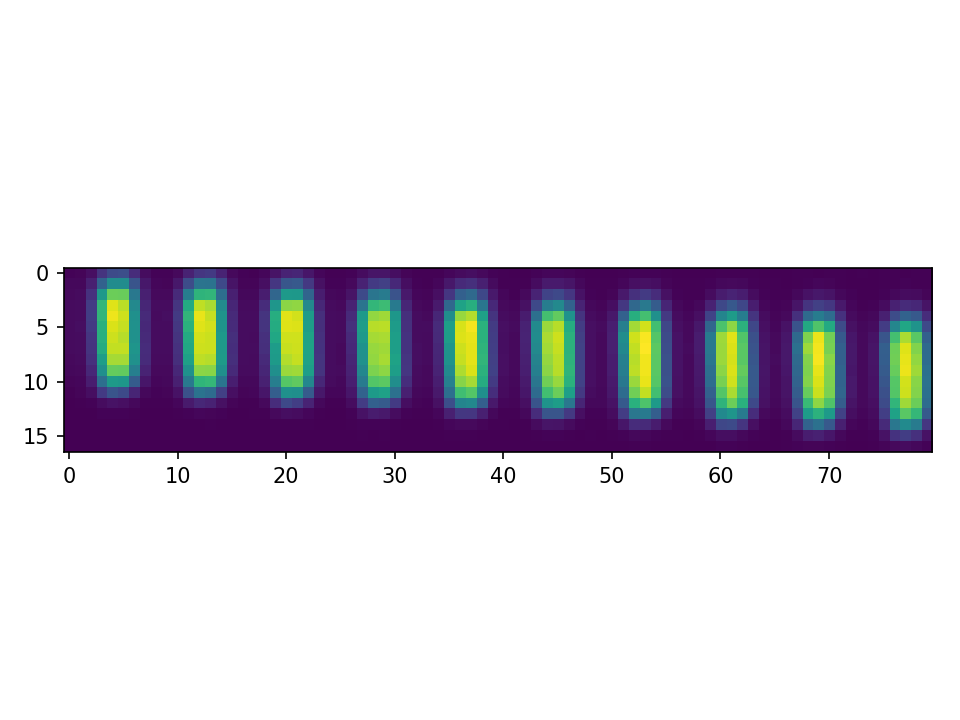
\includegraphics[width=0.49\textwidth]{img/maroonx_data.png}
    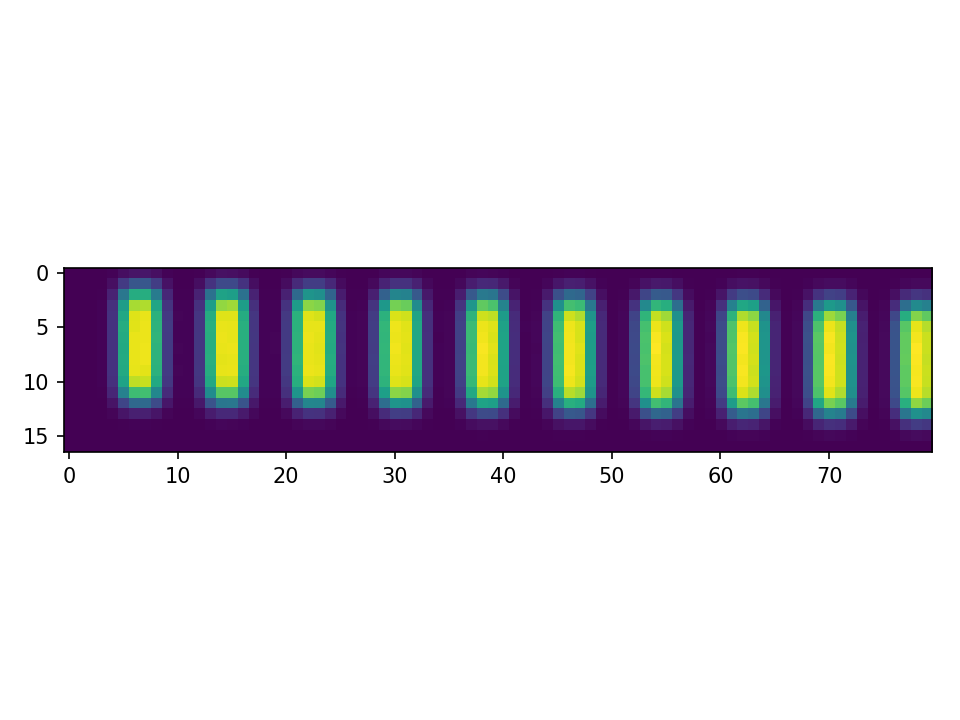
\includegraphics[width=0.49\textwidth]{img/simulator_data.png}
    \caption{Comparison between part of a recorded MaroonX etalon spectrum (left) and simulation data with a similar spectral format and source (right).}
\end{figure}

how the data are generated, what the tunable knobs are, maybe a figure comparing fake data to e.g. MAROON-X test data or HARPS?




details on the time-series spectra we generate

\subsection{Theoretical Information Content}
since we're generating the data ourselves, it's possible to calculate the \CRLB\ on how much \RV\ information is encoded in the spectrograph images.

\section{Methods}
\subsection{Optimal Extraction}
implementation details

\subsection{Spectro-perfectionism}
implementation details, with some discussion of the trickiest parts (e.g. getting the A matrix right)


\section{Results \& Discussion}
Here's what we get when we run our two methods on data generated under a variety of conditions.

First we show that under a variety of spectrograph configurations, even ones where optimal extraction fails, spectro-perfectionism performs well.

Then we address the issues with implementing spectro-perfectionism in the real world: insert reasonable levels of noise into the algorithm and see where/how it breaks.

\section{Conclusions}

summarize results: conditions under which spectro-perfectionism is a good option, conditions under which optimal extraction will do, and conditions under which they both break

emphasize that even if both algorithms break, the \RV\ content is still in the 2D spectrograph images! future outlook on 2D modeling to get \RV s WITHOUT extracting a spectrum.



\bibliographystyle{apj}
\bibliography{}%general,myref,inprep}

\end{document}